\documentclass[a4paper]{scrartcl}
\usepackage{amssymb, amsmath} % needed for math
\usepackage[utf8]{inputenc} % this is needed for umlauts
\usepackage[english]{babel} % this is needed for umlauts
\usepackage[T1]{fontenc}    % this is needed for correct output of umlauts in pdf
\usepackage[margin=2.5cm]{geometry} %layout
\usepackage{hyperref}   % links im text
\usepackage{braket}         % needed for \Set
\usepackage{parskip}
\usepackage[colorinlistoftodos]{todonotes}
\usepackage{pgfplots}
\pgfplotsset{compat=1.7,compat/path replacement=1.5.1}
\usepackage{tikz}

\title{Minimal distance to a cubic function}
\author{Martin Thoma}

\hypersetup{ 
  pdfauthor   = {Martin Thoma}, 
  pdfkeywords = {}, 
  pdftitle    = {Minimal Distance} 
}

\def\mdr{\ensuremath{\mathbb{R}}}

%%%%%%%%%%%%%%%%%%%%%%%%%%%%%%%%%%%%%%%%%%%%%%%%%%%%%%%%%%%%%%%%%%%%%
% Begin document                                                    %
%%%%%%%%%%%%%%%%%%%%%%%%%%%%%%%%%%%%%%%%%%%%%%%%%%%%%%%%%%%%%%%%%%%%%
\begin{document}
\maketitle
\begin{abstract}
In this paper I want to discuss how to find all points on a a cubic 
function with minimal distance to a given point.
\end{abstract}

\section{Description of the Problem}
Let $f: \mdr \rightarrow \mdr$ be a polynomial function and $P \in \mdr^2$
be a point. Let $d: \mdr^2 \times \mdr^2 \rightarrow \mdr_0^+$
be the euklidean distance of two points:
\[d \left ((x_1, y_1), (x_2, y_2) \right) := \sqrt{(x_1 - x_2)^2 + (y_1 - y_2)^2}\]

Now there is finite set of points $x_1, \dots, x_n$ such that 
\[\forall \tilde x \in \mathbb{R} \setminus \{x_1, \dots, x_n\}: d(P, (x_1, f(x_1))) = \dots = d(P, (x_n, f(x_n))) < d(P, (\tilde x, f(\tilde x)))\]

\section{Minimal distance to a constant function}
Let $f(x) = c$ with $c \in \mdr$ be a function. 

\begin{figure}[htp]
    \centering
    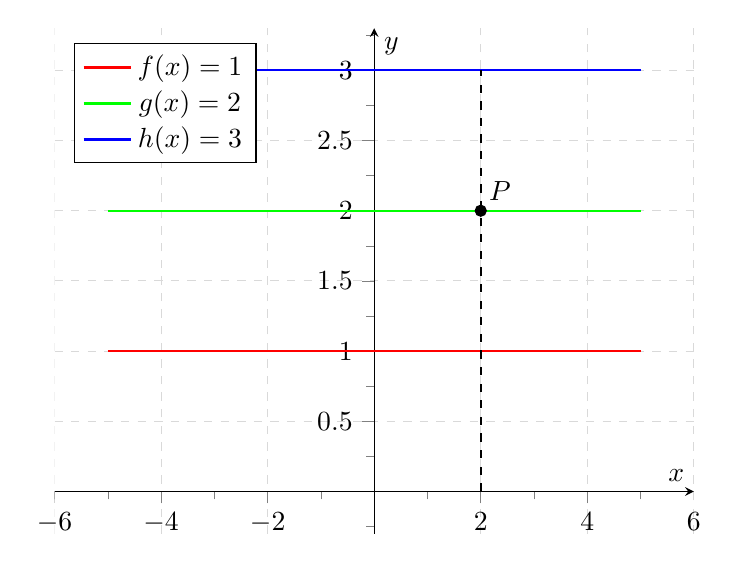
\begin{tikzpicture}
        \begin{axis}[
            legend pos=north west,
            axis x line=middle,
            axis y line=middle,
            grid = major,
            width=0.8\linewidth,
            height=8cm,
            grid style={dashed, gray!30},
            xmin=-5, % start the diagram at this x-coordinate
            xmax= 5, % end   the diagram at this x-coordinate
            ymin= 0, % start the diagram at this y-coordinate
            ymax= 3, % end   the diagram at this y-coordinate
            axis background/.style={fill=white},
            xlabel=$x$,
            ylabel=$y$,
            tick align=outside,
            minor tick num=-3,
            enlargelimits=true,
            tension=0.08]
          \addplot[domain=-5:5, thick,samples=50, red] {1};
          \addplot[domain=-5:5, thick,samples=50, green] {2};
          \addplot[domain=-5:5, thick,samples=50, blue] {3};
          \addplot[black, mark = *, nodes near coords=$P$,every node near coord/.style={anchor=225}] coordinates {(2, 2)};
          \draw[thick, dashed] (axis cs:2,0) -- (axis cs:2,3);
          \addlegendentry{$f(x)=1$}
          \addlegendentry{$g(x)=2$}
          \addlegendentry{$h(x)=3$}
        \end{axis} 
    \end{tikzpicture}
    \caption{3 constant functions}
\end{figure}

Then $(x_P,f(x_P))$ has
minimal distance to $P$. Every other point has higher distance.

\section{Minimal distance to a linear function}
Let $f(x) = m \cdot x + t$ with $m \in \mdr \setminus \Set{0}$ and 
$t \in \mdr$ be a function.

\begin{figure}[htp]
    \centering
    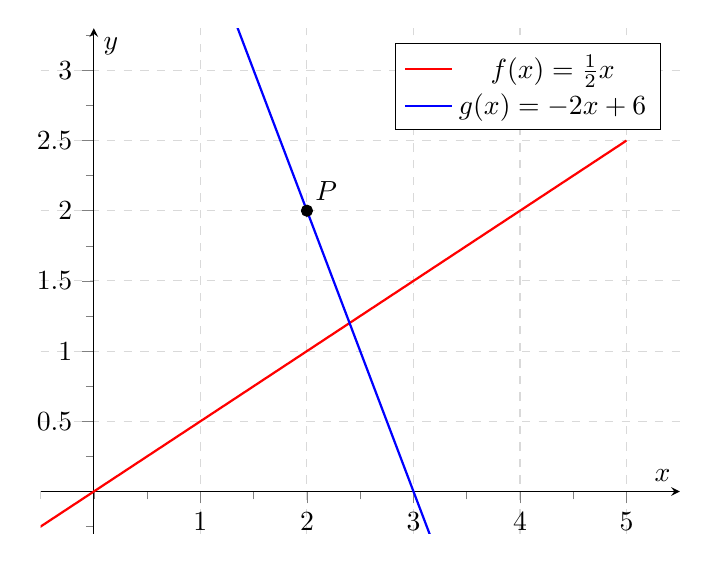
\begin{tikzpicture}
        \begin{axis}[
            legend pos=north east,
            axis x line=middle,
            axis y line=middle,
            grid = major,
            width=0.8\linewidth,
            height=8cm,
            grid style={dashed, gray!30},
            xmin= 0, % start the diagram at this x-coordinate
            xmax= 5, % end   the diagram at this x-coordinate
            ymin= 0, % start the diagram at this y-coordinate
            ymax= 3, % end   the diagram at this y-coordinate
            axis background/.style={fill=white},
            xlabel=$x$,
            ylabel=$y$,
            tick align=outside,
            minor tick num=-3,
            enlargelimits=true,
            tension=0.08]
          \addplot[domain=-5:5, thick,samples=50, red] {0.5*x};
          \addplot[domain=-5:5, thick,samples=50, blue] {-2*x+6};
          \addplot[black, mark = *, nodes near coords=$P$,every node near coord/.style={anchor=225}] coordinates {(2, 2)};
          \addlegendentry{$f(x)=\frac{1}{2}x$}
          \addlegendentry{$g(x)=-2x+6$}
        \end{axis} 
    \end{tikzpicture}
    \caption{The shortest distance of $P$ to $f$ can be calculated by using the perpendicular}
\end{figure}

Now you can drop a perpendicular through $P$ on $f(x)$. The slope $f_\bot$
of the perpendicular is $- \frac{1}{m}$. Then:

\begin{align}
                 f_\bot(x) &= - \frac{1}{m} \cdot x + t_\bot\\
    \Rightarrow        y_P &= - \frac{1}{m} \cdot x_P + t_\bot\\
    \Leftrightarrow t_\bot &= y_P + \frac{1}{m} \cdot x_P\\
    f(x) &= f_\bot(x)\\
    \Leftrightarrow m \cdot x + t &= - \frac{1}{m} \cdot x + \left(y_P + \frac{1}{m} \cdot x_P \right)\\
    \Leftrightarrow \left (m + \frac{1}{m} \right ) \cdot x &= y_P + \frac{1}{m} \cdot x_P - t\\
    \Leftrightarrow x &= \frac{m}{m^2+1} \left ( y_P + \frac{1}{m} \cdot x_P - t \right )
\end{align}

There is only one point with minimal distance.
\clearpage

\section{Minimal distance to a quadratic function}
Let $f(x) = a \cdot x^2 + b \cdot x + c$ with $a \in \mdr \setminus \Set{0}$ and 
$b, c \in \mdr$ be a function.

\begin{figure}[htp]
    \centering
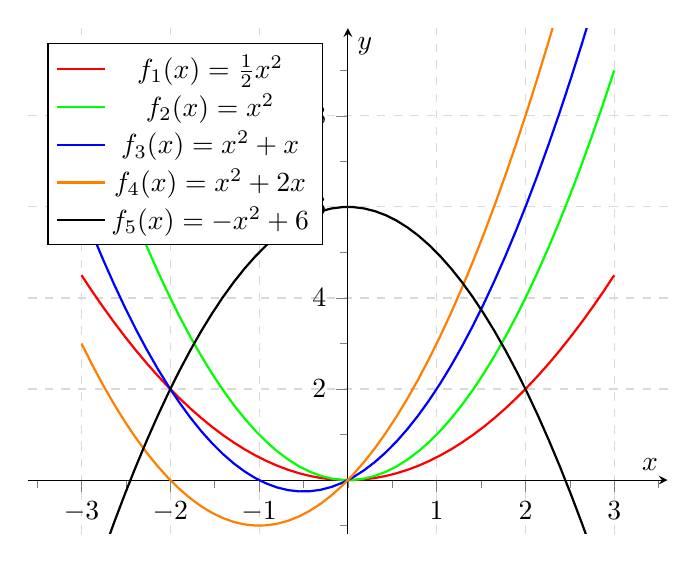
\begin{tikzpicture}
    \begin{axis}[
        legend pos=north west,
        axis x line=middle,
        axis y line=middle,
        grid = major,
        width=0.8\linewidth,
        height=8cm,
        grid style={dashed, gray!30},
        xmin=-3,     % start the diagram at this x-coordinate
        xmax= 3,    % end   the diagram at this x-coordinate
        ymin=-0.25,     % start the diagram at this y-coordinate
        ymax= 9,   % end   the diagram at this y-coordinate
        axis background/.style={fill=white},
        xlabel=$x$,
        ylabel=$y$,
        %xticklabels={-2,-1.6,...,7},
        %yticklabels={-8,-7,...,8},
        tick align=outside,
        minor tick num=-3,
        enlargelimits=true,
        tension=0.08]
      \addplot[domain=-3:3, thick,samples=50, red] {0.5*x*x}; 
      \addplot[domain=-3:3, thick,samples=50, green] {x*x}; 
      \addplot[domain=-3:3, thick,samples=50, blue] {x*x + x};
      \addplot[domain=-3:3, thick,samples=50, orange] {x*x + 2*x};
      \addplot[domain=-3:3, thick,samples=50, black] {-x*x + 6};
      \addlegendentry{$f_1(x)=\frac{1}{2}x^2$}
      \addlegendentry{$f_2(x)=x^2$}
      \addlegendentry{$f_3(x)=x^2+x$}
      \addlegendentry{$f_4(x)=x^2+2x$}
      \addlegendentry{$f_5(x)=-x^2+6$}
    \end{axis} 
\end{tikzpicture}
    \caption{Quadratic functions}
\end{figure}

\subsection{Number of points with minimal distance}
It is obvious that a quadratic function can have two points with 
minimal distance. 

For example, let $f(x) = x^2$ and $P = (0,5)$. Then $P_{f,1} \approx (2.179, 2.179^2)$
has minimal distance to $P$, but also $P_{f,2}\approx (-2.179, 2.179^2)$.

Obviously, there cannot be more than three points with minimal distance.
But can there be three points?

\begin{figure}[htp]
    \centering
    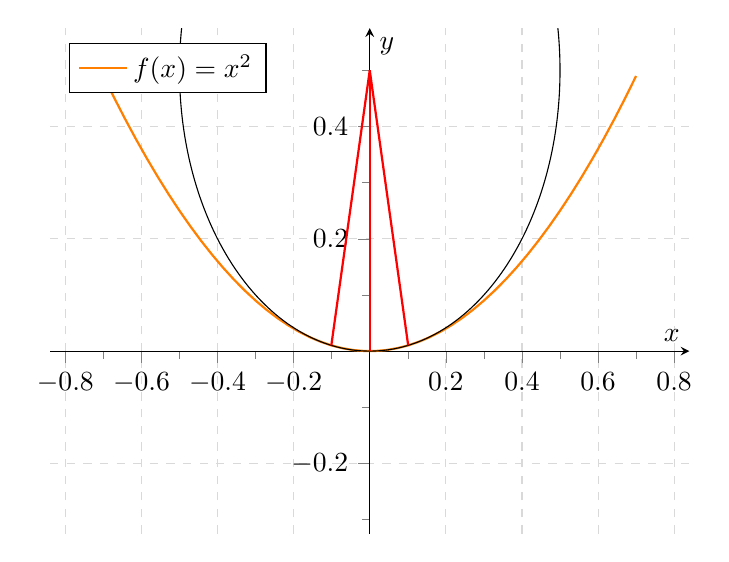
\begin{tikzpicture}
        \begin{axis}[
            legend pos=north west,
            axis x line=middle,
            axis y line=middle,
            grid = major,
            width=0.8\linewidth,
            height=8cm,
            grid style={dashed, gray!30},
            xmin=-0.7,     % start the diagram at this x-coordinate
            xmax= 0.7,    % end   the diagram at this x-coordinate
            ymin=-0.25,     % start the diagram at this y-coordinate
            ymax= 0.5,   % end   the diagram at this y-coordinate
            axis background/.style={fill=white},
            xlabel=$x$,
            ylabel=$y$,
            %xticklabels={-2,-1.6,...,7},
            %yticklabels={-8,-7,...,8},
            tick align=outside,
            minor tick num=-3,
            enlargelimits=true,
            tension=0.08]
          \addplot[domain=-0.7:0.7, thick,samples=50, orange] {x*x};
          \draw (axis cs:0,0.5) circle[radius=0.5];
          \draw[red, thick] (axis cs:0,0.5) -- (axis cs:0.101,0.0102);
          \draw[red, thick] (axis cs:0,0.5) -- (axis cs:-0.101,0.0102);
          \draw[red, thick] (axis cs:0,0.5) -- (axis cs:0,0);
          \addlegendentry{$f(x)=x^2$}
        \end{axis} 
    \end{tikzpicture}
    \caption{3 points with minimal distance?}
    \todo[inline]{Is this possible? http://math.stackexchange.com/q/553097/6876}
\end{figure}

\subsection{Calculate points with minimal distance}
\todo[inline]{Write this}

\section{Minimal distance to a cubic function}
Let $f(x) = a \cdot x^3 + b \cdot x^2 + c \cdot x + d$ with $a \in \mdr \setminus \Set{0}$ and 
$b, c, d \in \mdr$ be a function.

\subsection{Number of points with minimal distance}
\todo[inline]{Write this}

\subsection{Special points}
\todo[inline]{Write this}

\subsection{Voronoi}

For $b^2 \geq 3ac$

\todo[inline]{Write this}
\subsection{Calculate points with minimal distance}
\todo[inline]{Write this}
\end{document}
